\documentclass[spanish]{article}
\usepackage{graphicx}
\usepackage{ragged2e}
\usepackage{geometry}
\usepackage{float}
\usepackage{hyperref}
\usepackage[table,xcdraw]{xcolor}
\usepackage[ruled,vlined]{algorithm2e}
\title {Práctica 4: Divide y Venceŕas}
\graphicspath{{../img/}}
\addtolength{\textheight}{1.5in} 
\begin{document}
	\centerline{
\includegraphics[width=450px,height=100px]{header}}
	\centerline{Analisis de algoritmos, Sem: 2021-1, 3CV1,Práctica  3, 11/11/2020}
	\centering{\huge{Práctica 4: Divide y Vencéras}}
	\centerline{\newline{\textbf{Payán Téllez René}}}
	\newline{\textit{rpayant1500@alumno.ipn.mx}}
	\bigskip
	\justify
	\textbf{Resumen:}	
	En esta practica se analizaran 2 algoritmos que utilizan la tecnica de divide y venceras para resolver un problema, uno de ellos el quick sort y otro el sub arreglo maximo.\\
	\textbf{Palabras clave:}
	QuickSort,SubArreglo maximo,divide y venceras,C/C++
	\section{Introduccion}
	El saber implementar tecnicas de divide y venceras es fundamental para el desarrollo de algoritmos computacionales, ya que esta tecnica de resolver problemas abarca una enorme cantidad de algoritmos que resuelven problemas extremadamente complejos, o vitales para el funcionamiento de un sistema. En esta practica analizaremos a profundiad 2 de ellos QuickSort y MaxSubArray, tambien veremos como algunos de estos son afectados por las condiciones del problema y los compararemos con soluciones mas sencillas pero menos optimas.
	\section{Conceptos Basicos}
	\subsection{Algoritmo}
	La palabra algoritmo proviene del sobrenombre de un matemático árabe del siglo IX, Al-Khwarizmi, que fue reconocido por enunciar paso a paso las reglas para las operaciones matemáticas básicas con decimales (suma, resta, multiplicación y división).	
	Vemos definición de algoritmo como un grupo de órdenes consecutivas que presentan una solución a un problema o tarea. Algunos ejemplos de algoritmos los podemos encontrar en las matemáticas (como el algoritmo para resolver una multiplicación) y en los manuales de usuario de un aparato (como una lavadora o una impresora).	
	Sin embargo, hoy en día se relaciona la palabra algoritmo con el mundo de la informática, más concretamente en la programación; los conocidos como algoritmos informáticos.[1]
	\subsection{Divide y venceras}	
	El  término  Divide  y  Vencerás  en  su  acepción  más  amplia  es  algo  más  que  una  técnica  de  diseño  de  algoritmos.  De  hecho,  suele  ser  considerada  una  filosofía  general  para  resolver  problemas  y  de  aquí  que  su  nombre  no  sólo  forme  parte  del  vocabulario informático, sino que también se utiliza en muchos otros ámbitos.      En nuestro contexto, Divide y Vencerás es una técnica de diseño de algoritmos que  consiste  en  resolver  un  problema  a  partir  de  la  solución  de    del  mismo tipo, pero de menor tamaño. Si los subproblemas son todavía relativamente grandes   se   aplicará   de   nuevo   esta   técnica   hasta   alcanzar   subproblemas   lo   suficientemente  pequeños  para  ser  solucionados  directamente.  Ello  naturalmente  sugiere el uso de la recursión en las implementaciones de estos algoritmos.       La  resolución  de  un  problema  mediante  esta  técnica  consta  fundamentalmente  de los siguientes pasos: 1.   En   primer   lugar   ha   de   plantearse   el   problema   de   forma   que   pueda   ser   descompuesto  en  k  subproblemas  del  mismo  tipo,  pero  de  menor  tamaño.  Es  decir, si el tamaño de la entrada es n, hemos de conseguir dividir el problema en k  subproblemas  (donde  $1\leq k \leq n$),  cada  uno  con  una  entrada  de  tamaño  nk  y  donde $0\leq nk \leq n$. A esta tarea se le conoce como división. 2.    En    segundo    lugar    han    de    resolverse    independientemente    todos    los    subproblemas,  bien  directamente  si  son  elementales  o  bien  de  forma  recursiva.  El hecho de que el tamaño de los subproblemas sea estrictamente menor que el tamaño  original  del  problema  nos  garantiza  la  convergencia  hacia  los  casos  elementales, también denominados casos base. 3.  Por  último,  combinar las soluciones obtenidas en el paso anterior para construir la solución del problema original.[2]	
	\subsection*{QuickSort}	
	\begin{algorithm}[H]
		\KwData{Entrada: A[p,...,r]}
		\KwResult{Retorna la posicion del pivote i, un elemento que cumple con la propiedad de que todos los elementos desde p hasta i-1 son menores que A[i] y que de i+1 hasta r, todos los elementos son mayores que A[i]}
		x=A[r]\;
		i=p-1\;
		\For{$j\gets p$ \KwTo $j \leq r-1$}{
			\If{$A[j] \leq x$}{
				i++\;
				exchange(A[i],A[j]);
			}
		}
		exchange(A[i+1],A[r])\;
		return i+1\;
		\caption{Partition A[p,...,r]}
	\end{algorithm}
	\begin{algorithm}[H]
		\KwData{Entrada: A[p,...,n]}
		\KwResult{Retorna un areglo ordenado de forma ascendente}
		\If{$p < n$}{
			q=Partition(A,p,n)\;
			QuickSort(A,p,q-1)\;
			QuickSort(A,q+1,n)\;
		}
		\caption{QuickSort A[p,...,n]}
	\end{algorithm}
	\subsection*{Problema del maximo subarreglo}
	\begin{algorithm}[H]
		\KwData{Entrada: A[0,...,n-1], bajo, mitad, alto}
		\KwResult{Retorna la suma del mayor sub arreglo de la izquierda, la derecha y juntos}
		suma\textunderscore izq=INT\textunderscore  MIN\;
		suma=0\;
		max{\textunderscore}izq=0\;
		\For{$i\gets mitad\   \KwTo\   bajo$}{
			suma+=A[i]\;
			\If{$suma>suma\_izq$}{
				suma{\textunderscore}izq=suma\;
				max{\textunderscore}izq=i\;	
			}
		}
		suma{\textunderscore}der=INT{\textunderscore}MIN\;
		suma=0\;
		max{\textunderscore}der=0\;
		\For{$j\gets mitad\   \KwTo\   alto$}{
			suma+=A[j]\;
			\If{$suma>suma\_der$}{
				suma{\textunderscore}der=suma\;
				max{\textunderscore}der=j\;			
			}
		}
		return (max{\textunderscore}izq,max{\textunderscore}der,suma{\textunderscore}der+suma{\textunderscore}izq)\;
		\caption{MaxCrossingSubArray(A[0,...,n-1],bajo,mitad,alto)}		
	\end{algorithm}
	\begin{algorithm}[H]
		\KwData{Entrada: A[0,...,n-1], bajo, alto}
		\KwResult{retorna la suma y los indices del mayor sub arreglo, que se puede obtener dentro del arreglo A}
		\If{alto == bajo}{
			return(bajo,alto,A[bajo])\;
		}
		\Else{
			mitad=$\frac{bajo+alto}{2}$\;
			(bajo$\_$izq,alto$\_$izq,suma$\_$izq)=MaxSubArrayDC(A,bajo,mitad)\;
			(bajo$\_$der,alto$\_$der,suma$\_$der)=MaxSubArrayDC(A,mitad+1,alto)\;
			(cruz$\_$izq,cruz$\_$der,suma$\_$cruz)=MaxCrossingSubArray(A,bajo,mitad,alto)\;
			\If{$suma\_izq>suma\_der$\ and $suma\_izq>suma\_cruz$}{
				return (bajo$\_$izq,alto$\_$izq,suma$\_$izq)\;				
			}\ElseIf{$suma\_der>suma\_izq$\ and $suma\_der>suma\_cruz$}{
				return (bajo$\_$der,alto$\_$der,suma$\_$der)\;				
			}\Else{
				return (cruz$\_$izq,cruz$\_$der,suma$\_$cruz)\;
			}
		}		
		return (max{\textunderscore}izq,max{\textunderscore}der,suma{\textunderscore}der+suma{\textunderscore}izq)\;
		\caption{MaxSubArrayDC(A[0,...,n-1],bajo,alto)}
	\end{algorithm}
	\newpage
	\begin{algorithm}[H]
		\KwData{Entrada: A[0,...,n-1]}
		\KwResult{Retorna la suma y los indices del mayor sub arreglo, que se puede obtener dentro del arreglo A}
		sumaMaxima=$-\infty$\;
		indiceIzquierdo = 0\;
		indiceDerecho = 0\;
		\For{$i\gets 0\   \KwTo\   n$}{
			sumaLocal=0\;
			\For{$j\gets i\   \KwTo\   n$}{
				sumaLocal+=A[j]\;
				\If{sumaLocal$>$sumaMaxima}{
					sumaMaxima = sumaLocal\;
					indiceIzquierdo=i\;
					indiceDerecho=j\;
				}			
			}
		}
		return(sumaMaxima,indiceIzquierdo,indiceDerecho)\;
		\caption{FuerzaBruta(A[0,...,n-1])}
	\end{algorithm}
	\subsection*{Algoritmo de Karatsuba}	
	El algoritmo de Karatsuba es un algoritmo de multiplicación rápida . Fue descubierto por Anatoly Karatsuba en 1960 y publicado en 1962. Reduce la multiplicación de dos números de n dígitos a un máximo de multiplicaciones de un solo dígito en general (y exactamente cuando n es una potencia de 2). Por tanto, es más rápido que el algoritmo tradicional , que requiere productos de un solo dígito. Por ejemplo, el algoritmo de Karatsuba requiere 3 10 = 59,049 multiplicaciones de un solo dígito para multiplicar dos números de 1024 dígitos ( n = 1024 = 2 10 ), mientras que el algoritmo tradicional requiere (2 10 ) 2 = 1,048,576 (una aceleración de 17,75 veces).$n^{\log_2{3}} \approx n^{1.58}$.
	El algoritmo de Karatsuba fue el primer algoritmo de multiplicación asintóticamente más rápido que el algoritmo cuadrático de "escuela primaria". El algoritmo de Toom-Cook (1963) es una generalización más rápida del método de Karatsuba, y el algoritmo de Schönhage-Strassen (1971) es incluso más rápido, para n suficientemente grande.[3]
	\begin{algorithm}[H]
		\KwData{Entrada: $num_1$, $num_2$}
		\KwResult{retorna la multiplicacion de num1 y num2}
		\If{$num_1<$10 or $num_2<$10}{
			return $num_1$*$num_2$\;
		}
		m = min(longitud($num_1$),longitud($num_2$))\;
		$m_2$ = floor($\frac{m}{2}$)\;
		$alto_1$, $bajo_1$ = cortar($num_1$,$m_2$)\;
		$alto_2$, $bajo_2$ = cortar($num_2$,$m_2$)\;		
		$z_0$ = Karatsuba($bajo_1$, $bajo_2$)\;
		$z_1$ = Karatsuba(($bajo_1$ + $alto_1$),($bajo_2$ + $alto_2$))\;
		$z_2$ = Karatsuba($alto_1$, $alto_2$)\;
		return ($z_2*10^{2m_2}$+($z_1$-$z_2$-$z_0$)*$10^{m_2}$+$z_0$)
		\caption{Karatsuba($num_1$,$num_2$)}
	\end{algorithm}
	\section{Experimentacion y Resultados}
	\subsection{Implementar el algoritmo QuickSort.}
	Se ejecuto el programa para generar arreglos aleatorios de tamaño n (0$\rightarrow$100000) y ordenarlos mediante QuickSort.			
	\begin{figure}[h!]
		\centering
		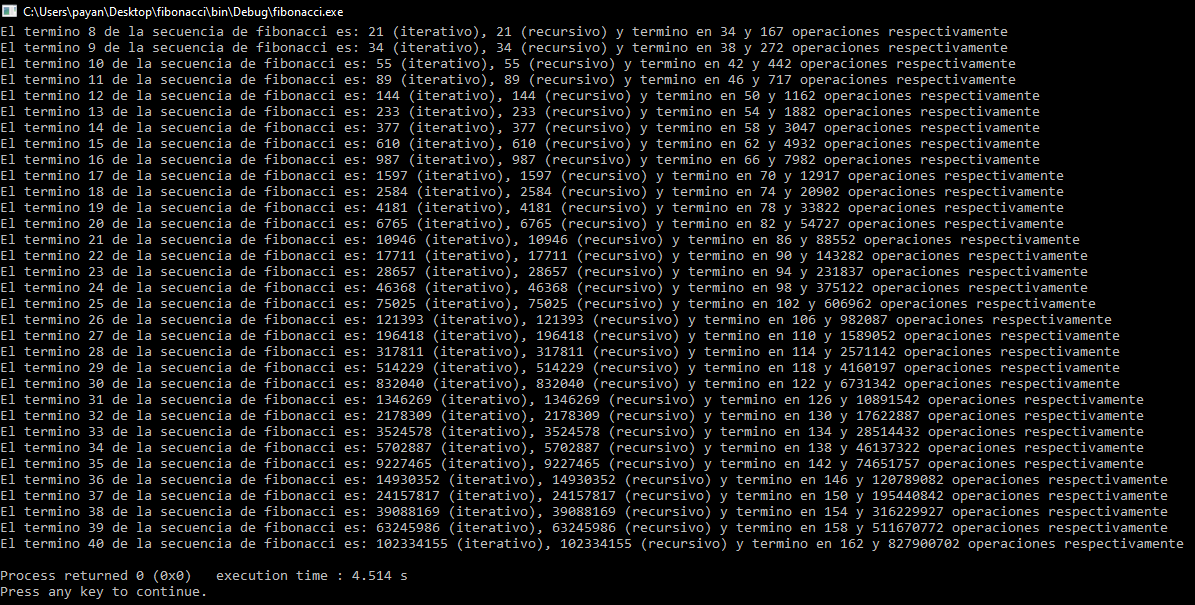
\includegraphics[width=400px,height=200px]{ejecucionPrimeraParte}
		\caption{Ejecucion del programa, Imprime el arreglo antes de ser ordenado y despues de ser ordenado, guarda en un archivo la cantidad de operaciones y el "n" para la funcion Partition (Se ejecuta en un arreglo aleatorio, aislado del ocupado por QuickSort), y los mismos datos pero para la funcion QuickSort.}
	\end{figure}
	\begin{figure}[H]
		\centering
		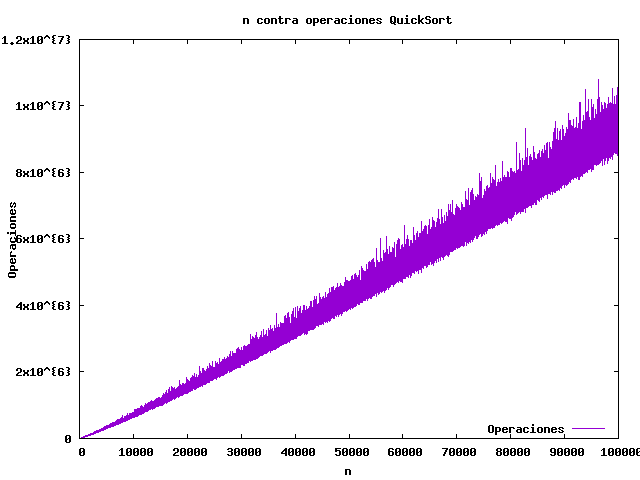
\includegraphics[width=400px,height=300px]{grafica1}
		\caption{N contra Operaciones de la funcion QuickSort en arreglos generados de forma aleatoria}
	\end{figure}
	\begin{figure}[H]
		\centering
		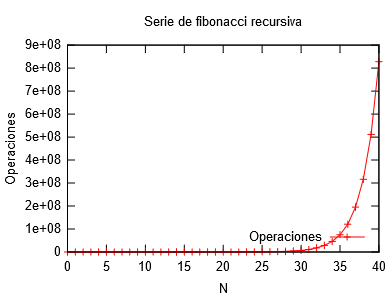
\includegraphics[width=400px,height=300px]{grafica2}
		\caption{N contra Operaciones de la funcion Partition en arreglos generados de forma aleatoria (No es el mismo arreglo que QuickSort)}
	\end{figure}	
	Ahora se procede a ejecutar la funcion QuickSort en un arreglo que contiene los numeros entre el 1 y n, donde n va desde 2 hasta 10000 ordenados de 4 formas distintas. Siendo estas:\
	\begin{enumerate}
		\item Esta ordenado de forma ascendente. Ejemplo: 1,2,3,4
		\item Esta ordenado de forma descendente. Ejemplo: 4,3,2,1
		\item Esta ordenado de forma aleatoria. Ejemplo: 2,4,1,3
		\item Esta ordenado de forma que el pivote corte el arreglo a la mitad, es decir la primera mitad del arreglo de forma ascendente y la siguiente de forma descendente. Ejemplo: 1,2,4,3
	\end{enumerate}
	\begin{figure}[H]
		\centering
		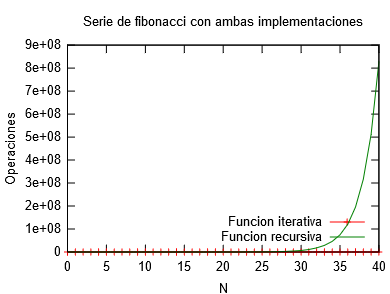
\includegraphics[width=400px,height=300px]{grafica3}
		\caption{N contra Operaciones del caso 1 de QuickSort}
	\end{figure}	
	\begin{figure}[H]
		\centering
		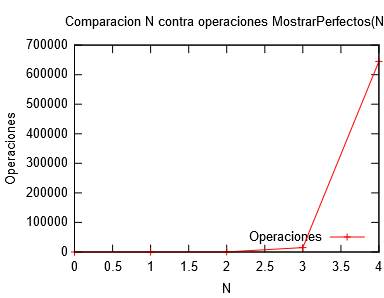
\includegraphics[width=400px,height=300px]{grafica4}
		\caption{N contra Operaciones del caso 2 de QuickSort}
	\end{figure}	
	\begin{figure}[H]
		\centering
		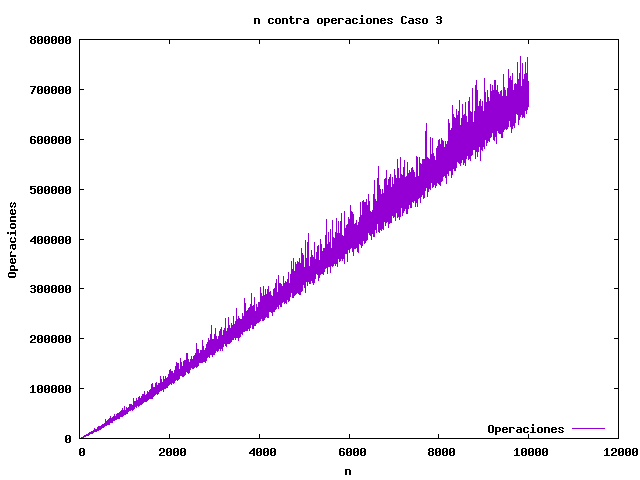
\includegraphics[width=400px,height=300px]{grafica5}
		\caption{N contra Operaciones del caso 3 de QuickSort}
	\end{figure}	
	\begin{figure}[H]
		\centering
		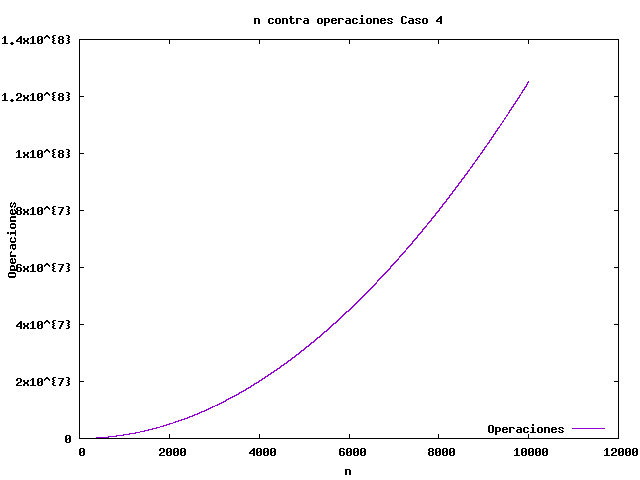
\includegraphics[width=400px,height=300px]{grafica6}
		\caption{N contra Operaciones del caso 4 de QuickSort}
	\end{figure}	
	\begin{figure}[H]
		\centering
		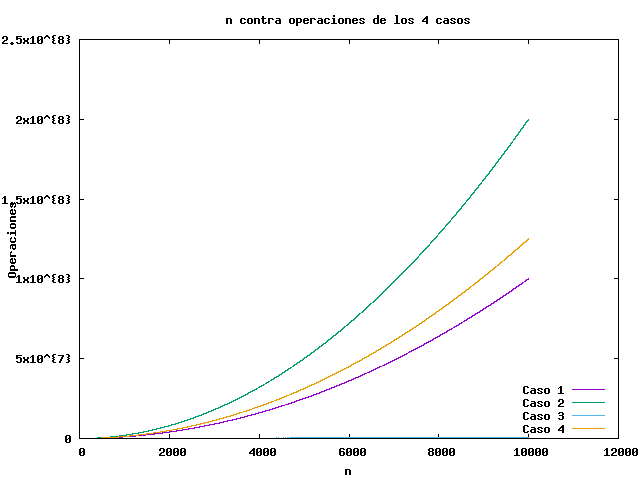
\includegraphics[width=400px,height=300px]{grafica7}
		\caption{N contra Operaciones de todos los casos combinados de QuickSort}
	\end{figure}	
	Ahora procedemos a calcular formalmente la complejidad de la funcion Partition
	Empezamos calculando la complejidad temporal de cada linea:
	\begin{center}
		\begin{table}[H]
			\begin{tabular}{|l|l|l|}
				\hline
				\rowcolor[HTML]{FFCC67} 
				Codigo                           & Costo & Veces ejecutado \\ \hline
				\textit{x = A[hasta]}                    & $\O(1)$    & 1               \\ \hline
				\textit{i = desde-1}                    & $\O(1)$    & 1               \\ \hline
				\textit{for(j=desde;j$<$hasta;j++)} & $\O(n)$    & n+1             \\ \hline
				\textit{\  \  if(A[j]<i)}                 & $\O(1)$    & n               \\ \hline
				\textit{\  \  \  \  i++}                     & $\O(1)$    & desconocido               \\ \hline
				\textit{\  \  \  \  intercambiar(A[i],A[j])}                     & $\O(3)$    & desconocido               \\ \hline
				\textit{intercambiar(A[i+1],A[hasta])}                     & $\O(3)$    & 1               \\ \hline
				\textit{return i+1}                & $\O(1)$    & 1               \\ \hline
			\end{tabular}
		\end{table}										
	\end{center}
	Esto nos indica que la complejidad de la funcion partition se ve determinada por el for que recorre desde 0 hasta n y como no es posible calcular la cantidad de veces que entrara dentro del if (ya que esto dependera del pivote), y apoyandonos por la Figure 3, podemos concluir que la funcion partition tiene complejidad $\O(n)$.\\			
	Ahora procedemos a calcular formalmente la complejidad de la funcion QuickSort (suponiendo que el pivote corta en medio del arreglo)
	Empezamos calculando la complejidad temporal de cada linea:
	\begin{center}
		\begin{table}[H]
			\begin{tabular}{|l|l|l|}
				\hline
				\rowcolor[HTML]{FFCC67} 
				Codigo                           & Costo & Veces ejecutado \\ \hline
				\textit{if(desde < hasta)}                    & $\O(1)$    & 1               \\ \hline
				\textit{\  \  q = Partition(A,desde,hasta)}                    & $\O(n)$    & 1               \\ \hline
				\textit{\  \  QuickSort(A,desde,q-1)}                    & $T(\frac{n}{2})$    & 1               \\ \hline						
				\textit{\  \  QuickSort(A,q+1,hasta)}                    & $T(\frac{n}{2})$    & 1               \\ \hline						
			\end{tabular}
		\end{table}										
	\end{center}
	Bajo este escenario que coincide con el caso 4 de los analisis respecto a QuickSort (Figure 7) obtenemos la siguiente ecuacion de recurrencia:\\
	$T(n) = 2T(\frac{n}{2})+\O(n)$\\
	Que al ser desarrollada llegaremos a la conclusion de que: $T(n)$ tiene complejidad $\Theta(nlog_2(n))$.\\
	Ahora bien, para los otros 3 escenarios la cosa cambia bastante, si miramos la figure 4 podemos ver que el comportamiento de la funcion se torna cuadratico, muy similar al escenario 2 (Figure 5), ya que generamos casos donde el arreglo es dividido en 0 y n elementos, lo cual vuelve la complejidad del ordenamiento cuadratica.\\
	Pero tomando el caso de números aleatorios (Figure 6 y Figure 2) podemos ver que en la mayoria de los casos, el algoritmo tendra complejidad $\O(nlog_2(n))$, aunque dependera de la implementación, en este caso se tomo el pivote como el ultimo valor del arreglo, lo cual es puede ser poco eficiente, por ello se recomienda tomar valores como la media o mediana.\\
	\subsection{Implementar el algoritmo del Maximo SubArreglo}
	Para este algoritmo se decidio generar un arreglo aleatorio de n elementos (n va de 1 hasta 10000), y medir la complejidad del algoritmo de fuerza bruta y del algoritmo de divide y venceras.
	\begin{figure}[H]
		\centering
		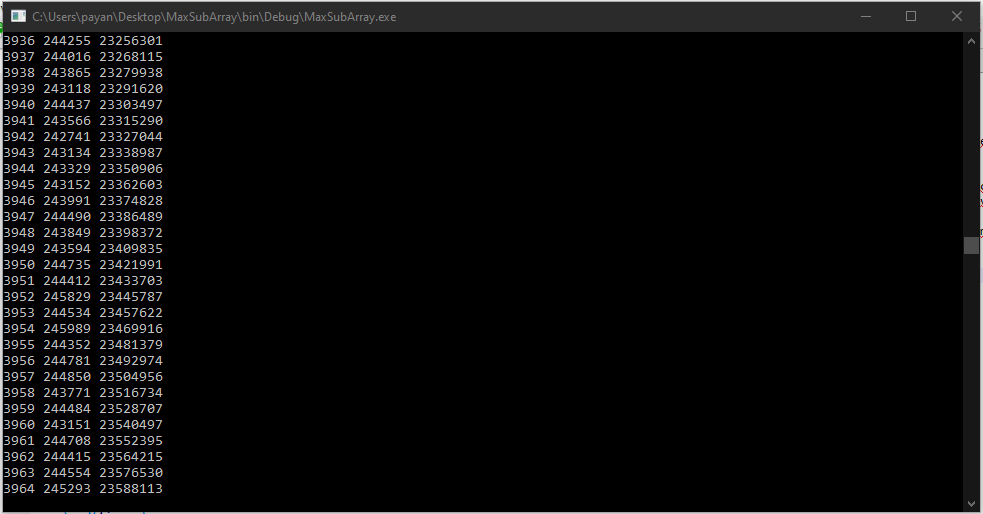
\includegraphics[width=400px,height=200px]{ejecucionSegundaParte}
		\caption{Ejecucion del programa en la seccion de prueba de números}
	\end{figure}
	\begin{figure}[H]
		\centering
		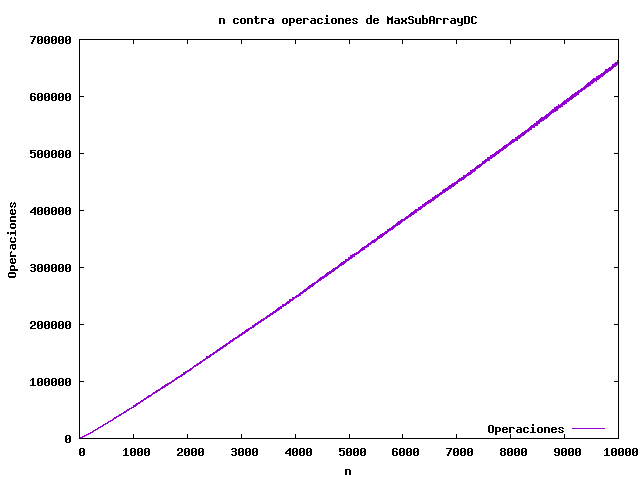
\includegraphics[width=400px,height=300px]{grafica8}
		\caption{N contra Operaciones de MaxSubArrayDC en arreglos aleatorios de tamaño n}
	\end{figure}
	\begin{figure}[H]
		\centering
		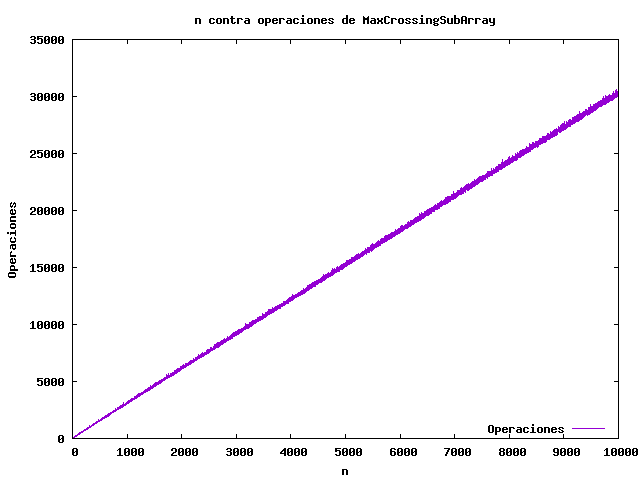
\includegraphics[width=400px,height=300px]{grafica9}
		\caption{N contra Operaciones de MaxCrossingSubArray en arreglos aleatorios de tamaño n}
	\end{figure}
	\begin{figure}[H]
		\centering
		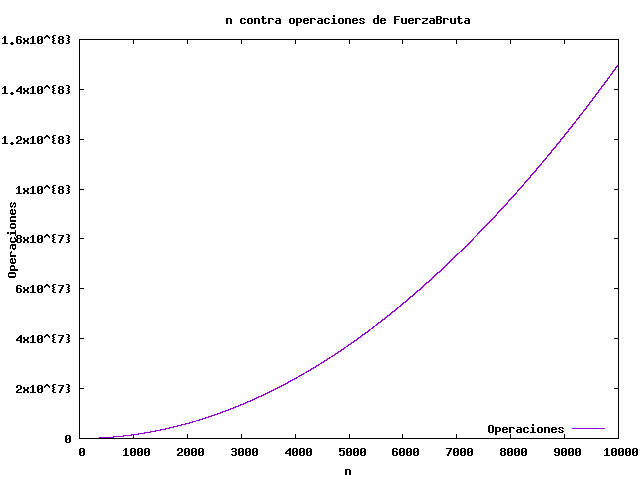
\includegraphics[width=400px,height=300px]{grafica10}
		\caption{N contra Operaciones de FuerzaBruta en arreglos aleatorios de tamaño n}
	\end{figure}
	\begin{figure}[H]
		\centering
		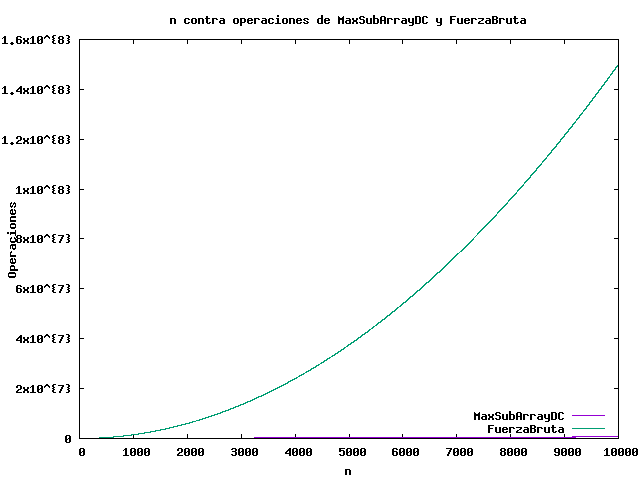
\includegraphics[width=400px,height=300px]{grafica11}
		\caption{N contra Operaciones de MaxSubArrayDC y FuerzaBruta combinados en arreglos aleatorios de tamaño n}
	\end{figure}
	Ahora procederemos a calcular formalmente la complejidad de la funcion MaxCrossingSubArray:
	\begin{center}
		\begin{table}[H]
			\begin{tabular}{|l|l|l|}
				\hline
				\rowcolor[HTML]{FFCC67} 
				Codigo                           & Costo & Veces ejecutado \\ \hline
				\textit{suma, suma$\_$izq, suma$\_$der}                    & $\O(1)$    & 1               \\ \hline
				\textit{max$\_$izq = max$\_$der = INT$\_$MIN;}                    & $\O(1)$    & 1               \\ \hline								
				\textit{for(i=mitad;i$\geq$bajo;i--)} & $\O(1)$    & $\frac{n}{2}+1$             \\ \hline
				\textit{\  \  suma+=arreglo[i]}                 & $\O(1)$    & $\frac{n}{2}$               \\ \hline
				\textit{\  \  if(suma$>$suma$\_$izq)}                 & $\O(1)$    & $\frac{n}{2}$               \\ \hline
				\textit{\  \  \  \  max$\_$izq=i}                     & $\O(1)$    & indefinido              \\ \hline
				\textit{\  \  \  \  suma$\_$izq=suma}                     & $\O(1)$    & indefinido              \\ \hline				
				\textit{for(i=mitad+1;i$<$alto;i++)} & $\O(1)$    & $\frac{n}{2}$+1             \\ \hline
				\textit{\  \  suma+=arreglo[i]}                 & $\O(1)$    & $\frac{n}{2}$               \\ \hline
				\textit{\  \  if(suma$>$suma$\_$der)}                 & $\O(1)$    & $\frac{n}{2}$               \\ \hline
				\textit{\  \  \  \  max$\_$der=i}                     & $\O(1)$    & indefinido              \\ \hline
				\textit{\  \  \  \  suma$\_$der=suma}                     & $\O(1)$    & indefinido              \\ \hline			
				\textit{return(suma$\_$izq+suma$\_$der,max$\_$izq,max$\_$der)}                     & $\O(1)$    & 1              \\ \hline			
			\end{tabular}
		\end{table}										
	\end{center}			
	Al analizar la complejidad linea a linea y apoyado por la grafica "Figure 11" , podemos decir que la complejidad de la funcion es $O(n)$.
	Una vez que tenemos este dato, procedemos a analizar la complejidad de la funcion MaxSubArrayDC:
	\begin{center}
		\begin{table}[H]
			\begin{tabular}{|l|l|l|}
				\hline
				\rowcolor[HTML]{FFCC67} 
				Codigo                           & Costo & Veces ejecutado \\ \hline
				\textit{suma, suma$\_$izq, suma$\_$der}                    & $\O(1)$    & 1               \\ \hline
				\textit{max$\_$izq = max$\_$der = INT$\_$MIN;}                    & $\O(1)$    & 1               \\ \hline								
				\textit{for(i=mitad;i$\geq$bajo;i--)} & $\O(1)$    & $\frac{n}{2}+1$             \\ \hline
				\textit{\  \  suma+=arreglo[i]}                 & $\O(1)$    & $\frac{n}{2}$               \\ \hline
				\textit{\  \  if(suma$>$suma$\_$izq)}                 & $\O(1)$    & $\frac{n}{2}$               \\ \hline
				\textit{\  \  \  \  max$\_$izq=i}                     & $\O(1)$    & indefinido              \\ \hline
				\textit{\  \  \  \  suma$\_$izq=suma}                     & $\O(1)$    & indefinido              \\ \hline				
				\textit{for(i=mitad+1;i$<$alto;i++)} & $\O(1)$    & $\frac{n}{2}$+1             \\ \hline
				\textit{\  \  suma+=arreglo[i]}                 & $\O(1)$    & $\frac{n}{2}$               \\ \hline
				\textit{\  \  if(suma$>$suma$\_$der)}                 & $\O(1)$    & $\frac{n}{2}$               \\ \hline
				\textit{\  \  \  \  max$\_$der=i}                     & $\O(1)$    & indefinido              \\ \hline
				\textit{\  \  \  \  suma$\_$der=suma}                     & $\O(1)$    & indefinido              \\ \hline			
				\textit{return(suma$\_$izq+suma$\_$der,max$\_$izq,max$\_$der)}                     & $\O(1)$    & 1              \\ \hline			
			\end{tabular}
		\end{table}										
	\end{center}
	Terminado el analisis, obtendremos que la complejidad esta determinada por la siguiente ecuacion de recurrencia: $T(n) = 2T(\frac{n}{2})+\O(n)$, una vez resuelta, determinaremos que la complejidad final de la funcion MaxSubArrayDC es $\O(nlog_2(n))$ esto lo podemos respaldar con las Figure 10 y Figure 13 , en las cuales se aprecia que la complejidad de la funcion esta acotada por $\O(nlog_2(n))$.
	Finalmente como contraste se analizara la funcion FuerzaBruta:
	\begin{center}
		\begin{table}[H]
			\begin{tabular}{|l|l|l|}
				\hline
				\rowcolor[HTML]{FFCC67} 
				Codigo                           & Costo & Veces ejecutado \\ \hline
				\textit{sumaLocal, lIndex, rIndex = 0}                    & $\O(1)$    & 1               \\ \hline
				\textit{suma = INT$\_$MAX}                    & $\O(1)$    & 1               \\ \hline				

				\textit{for(i=0;i$<$n;i++)} & $\O(1)$    & $n+1$             \\ \hline
				\textit{\  \  sumaLocal=0}                 & $\O(1)$    & $n$               \\ \hline
				\textit{\  \  for(j=i;j$<$n;j++)}                 & $\O(1)$    & $n$               \\ \hline
				\textit{\  \  \  \  if(sumaLocal$>$suma)}                     & $\O(1)$    & $\frac{(n)(n-1)}{2}+1$              \\ \hline
				\textit{\  \  \  \  \  \  suma = sumaLocal}                     & $\O(1)$    & indefinido              \\ \hline				
				\textit{\  \  \  \  \  \  lIndex = i}                     & $\O(1)$    & indefinido              \\ \hline				
				\textit{\  \  \  \  \  \  rIndex = j}                     & $\O(1)$    & indefinido              \\ \hline								
				\textit{return(suma,lIndex,rIndex)}                     & $\O(1)$    & 1              \\ \hline			
			\end{tabular}
		\end{table}										
	\end{center}
	Al terminar el analisis podemos ver que la complejidad de la funcion es $\O(n^2)$ lo cual coincide bastante con lo que se aprecia en las graficas (Figure 12 y Figure 13).

	
	\section{Conclusiones}			
	\subsection{Payán Téllez René}
	Despues de analizar los algoritmos del maximo sub arreglo y del QuickSort, puedo concluir que la tecnica de divide y venceras es extremadamente potente y sirve para resolver problemas que de otra forma tomarian mucha mas complejidad computacional, por ejemplo la funcion FuerzaBruta y el BubbleSort son prueba de ello ya que estos algoritmos que implementan soluciones mas directas, tienen complejidades enormes. Por otro lado no todo es perfecto, ya que en el caso particular del QuickSort, pude apreciar que la complejidad podia crecer hasta ser extremadamente ineficiente en casos donde el arreglo este ordenado de tal forma que el pivote no corte nada del mismo, aunque analizando a profundidad estos casos pueden ser diezmados y en ciertas implementaciones que me encontre en la web, se toman varias medidas para hacerlo, como aleatorizar el arreglo o buscar un pivote mas optimo.\\
	\includegraphics[height=120px,width=120px]{Rene}
	\section{Anexo}			
	\subsection{Investigar el algoritmo de Karatsuba que permite obtener la multiplicación de enteros muy grandes}
	Resuelto, se encuentra en los conceptos basicos
	\subsection{Resolver los siguientes problemas}
	\section{Bibliografia}
		{[}1{]}\url{https://openwebinars.net/blog/que-es-un-algoritmo-informatico/}\\
		{[}2{]}\url{http://www.lcc.uma.es/~av/Libro/CAP3.pdf}\\
		{[}3{]}\url{https://es.qaz.wiki/wiki/Karatsuba_algorithm}\\
	\end{document}